\documentclass[11pt]{article}
\usepackage{amsmath, amssymb}
\usepackage{graphicx}
\usepackage{float}
\usepackage{hyperref}
\usepackage{enumitem}
\usepackage{booktabs}
\usepackage{multirow}
\usepackage[margin=1in]{geometry}

\title{Survey of Algorithms Applied to the Traveling Salesman Problem \\ under Deadline Constraints}
\author{Alles Rebel}
\date{\today}

\begin{document}
	\maketitle
	
	\begin{abstract}
		This report presents a comprehensive survey of several algorithms applied to the well-known Traveling Salesman Problem (TSP) with a focus on deadline constraints. We compare heuristic based and local search based methodologies, and analyze their performance under various time restrictions using datasets from TSPLIB95. Particular attention is given to whether each method improves incrementally with additional time or requires a complete, node-by-node construction to yield a valid solution. We propose a framework to convert complete exploration algorithm to an all time algorithm suitable for use with time constraints.
	\end{abstract}
	
	\section{Introduction}
	The Traveling Salesman Problem (TSP) is a classical optimization problem in which a salesman must visit a set of cities exactly once and return to the origin city while minimizing the total travel cost. Due to its \textbf{NP-hard} nature, numerous approaches have been proposed over the years, ranging from simple heuristics to complex stochastic algorithms. In real-world applications, time constraints (or deadlines) are common, and these algorithms must deliver good solutions within limited computational time. This report surveys several algorithms and proposes an augmentation with the goal of understanding which techniques are best suited when runtime is a critical factor, and how solution quality is affected by additional computational time across data space exploration.
	
	\section{Problem Definition}
	Given a set of $n$ cities and a cost function (distance matrix) between each pair of cities, the objective is to determine a permutation of the cities that minimizes the total tour cost. The dataset used for our experiments is taken from \texttt{https://people.sc.fsu.edu/~jburkardt/datasets/tsp/tsp.html}\cite{Dataset}, which provides TSPLIB95-compatible\cite{TSPLIB} data along with known optimal solutions.
	
	\section{Dataset Details}
	The experimental datasets are TSPLIB95 instances obtained from \url{https://people.sc.fsu.edu/~jburkardt/datasets/tsp/tsp.html}. Each file contains the following elements:
	\begin{itemize}[noitemsep]
		\item \textbf{Header Information:} Includes the instance name, type (typically \texttt{TSP}), comments, and the \texttt{DIMENSION} field that specifies the number of cities.
		\item \textbf{Edge Weight Type:} Indicates how the distance between cities is computed (e.g., \texttt{EUC\_2D} for Euclidean distances in 2D space).
		\item \textbf{Node Coordinates Section:} A listing of each city's index and its corresponding x and y coordinates. These coordinates are used to compute the distances among cities.
		\item \textbf{Known Optimal Solutions:} Many instances include or are accompanied by the known optimal tour cost, which is used as a benchmark to evaluate the performance of various algorithms.
	\end{itemize}
	
	The dataset files used in our experiments are as follows. Note that the number in each file name generally indicates the number of cities in that instance:
	
	\begin{table}[H]
		\centering
		\begin{tabular}{lccc}
			\toprule
			Instance File    & Number of Cities & Known Optimal Cost \\
			\midrule
			att48.tsp      & 48              & 10628 \\
			dantzig42.tsp  & 42              & 699 \\
			fri26.tsp      & 26              & 937 \\
			gr17.tsp       & 17              & 2085 \\
			p01.tsp        & 15              & 291 \\
			\bottomrule
		\end{tabular}
		\caption{List of TSPLIB instance files and their known optimal costs.}
		\label{table:tsplib}
	\end{table}
	
	\section{Algorithmic Approaches}
	In this survey, we examine algorithms from two main categories:
	
	\subsection{Heuristic-Based Approaches}
	Heuristic algorithms are strategies that seek to produce good-quality solutions within a reasonable time by leveraging rules-of-thumb or domain-specific knowledge. Unlike exact methods that guarantee an optimal solution but may be computationally expensive, heuristics provide approximate answers that are often “good enough” for practical purposes. They are particularly valuable under tight deadline constraints because they can quickly generate a complete solution, even if that solution is not optimal. However, most heuristic algorithms do not refine their results iteratively once an initial solution is produced; so additional computational time may not yield significant improvements.
	
	\subsubsection{Simple Minimum Distance}
	The \textbf{Minimum Distance} heuristic (or greedy algorithm) selects the nearest unvisited city at each step. This greedy approach produces a complete solution almost instantly; however, it does not refine its solution iteratively. In other words, providing additional time beyond the initial solution does not improve the outcome. The simplicity of this algorithm is attractive for extremely tight deadlines, though the resulting tour is typically suboptimal compared to more sophisticated methods.
	
	\subsubsection{Graph Based A* Search + Augmentation}
	A* search is a well-known graph traversal and pathfinding algorithm \cite{4082128} that employs a heuristic function to estimate the cost from the current node to the goal. For TSP, a minimum spanning tree (MST) of the remaining nodes—to guide the search is used as the heuristic. Although A* can theoretically be interrupted to provide a partial solution, it is generally not considered an any time algorithm because a valid, fully optimal solution is only available after the complete search has been conducted. 
	
	In this work, we improve the original algorithm's performance with time constraints; the best partial solution computed is completed using Simple Minimum Distance heuristic to produce a valid tour from the best solution discovered. This allows the traditional A* algorithm to function as an any time algorithm.
	
	\subsubsection{Tree Based Branch and Bound with MST}
	The \textbf{Branch and Bound} method\cite{MORRISON201679} systematically enumerates candidate tours and prunes paths where the lower bound—often derived from the MST cost of the remaining nodes—exceeds the current best solution. Like A*, this method constructs the solution node by node and only provides a complete solution once the search is finished. However, like simple heuristic search, it's an extremely fast algorithm. And an excellent candidate to augment slower accurate methods when time constraints are considered.
	
	\subsection{Local Search-Based Approaches}
	Local search algorithms are iterative methods that start from an initial solution and improve it by exploring the neighborhood of that solution. In this context, the "neighborhood" consists of solutions that are reachable by making small modifications (e.g., swapping two cities in the tour). These methods are categorized as anytime algorithms since they always yield a valid solution and can progressively enhance solution quality as more computation time is provided. However, a common challenge for local search is the risk of getting trapped in local optima, where no small change results in an improvement. To mitigate this, techniques such as random restarts, perturbation, or other inspired enhancements (e.g., simulated annealing or genetic operators) are often incorporated.
	
	\subsubsection{Standard Local Search}
	Standard local search iteratively improves a candidate solution by exploring its neighborhood. The variant implemented for this work is known as $2-opt$ Local Search, applied to the Generalized Traveling Salesman problem \cite{DIMITRIJEVIC1997105}. Conceptually simple, while exploring the neighborhood, the algorithm simply notes improvements and chooses the best improvement, which may result in getting stuck in a local minima. In contrast to the next few methods which deal with local minima by introducing randomness into this selection process. Given enough time, the algorithm can progressively escape shallow local minima. Note, this algorithm does not require any hyper parameters.
	
	\subsubsection{Genetic Algorithm}
	Genetic Algorithms (GAs) are population-based sampling of the solution space that simulate the process of natural evolution. They involve selection, crossover, and mutation operators to evolve a set of candidate solutions over multiple generations\cite{wikipedia_genetic_algorithm}. GAs are naturally anytime algorithms; they always maintain a population of complete solutions that improve as more computational time is allocated. However, the quality of improvements depends on proper parameter tuning (e.g., crossover and mutation rates) and the convergence characteristics of the population.
	
	\subsubsection{Simulated Annealing}
	Simulated Annealing (SA) employs a probabilistic acceptance criterion that allows for occasional uphill moves to escape local optima\cite{wikipedia_simulated_annealing}. SA starts with a complete solution and gradually improves it by accepting changes based on a cooling schedule. To avoid local minima, lower scoring or uphill neighbors are sometimes kept depending on the temperature. This selection of lower scoring neighbors is significantly reduced as the temperature drops or is cooled down. As an anytime algorithm, SA always provides a valid solution, with quality generally improving with more iterations—up to the point where the temperature becomes too low to allow further meaningful changes.
	
	\section{Experimental Setup}
	The experimental setup involves running each solver on a desktop computer equipped with a multi-threaded processor. Each algorithm is implemented as a separate thread, ensuring that all solvers work with the same dataset and starting position. Experiments were conducted on the five TSPLIB95 instances listed in Table~\ref{table:tsplib}. For each dataset, various deadlines were imposed, ranging from a second to minutes. And each individual time control or deadline, was run multiple times to collect a statistical distribution. This helps control variation in performance due to randomness inherent in a operating system's scheduling or caching. To further insure additional bias was avoided, each trial configuration was shuffled prior to assignment to random thread. Threads were limited to number of threads the processor architecture supported.
	Performance metrics include the quality of the solution (measured as the deviation from the known optimal cost), computational time, and consistency across runs. Special emphasis was placed on understanding whether additional time leads to incremental improvements (as with anytime algorithms) or if a method must complete a full, node-by-node construction before yielding a valid solution.
	
	\section{Experimental Results}
	
	\begin{figure}[H]
		\centering
		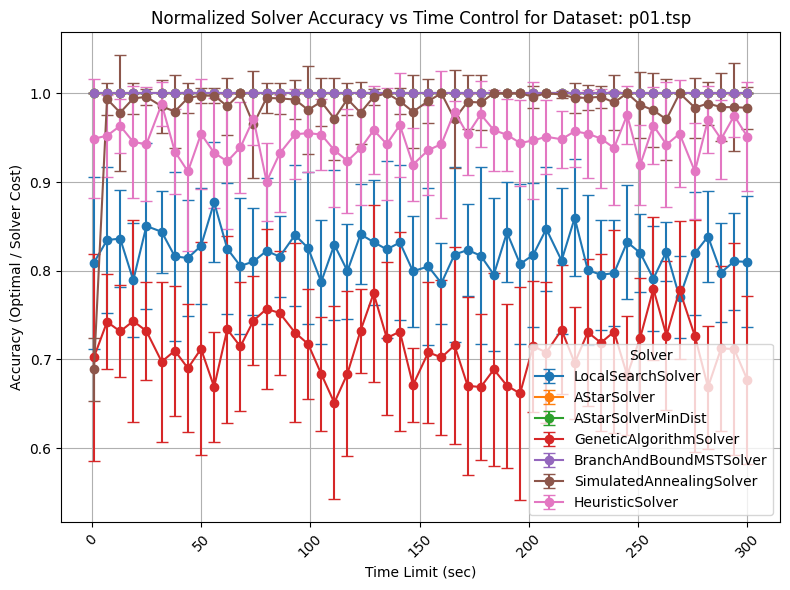
\includegraphics[width=0.7\linewidth]{figures/accuracy_line_p01.tsp}
		\caption{}
		\label{fig:accuracylinep01}
	\end{figure}
	\begin{figure}[H]
		\centering
		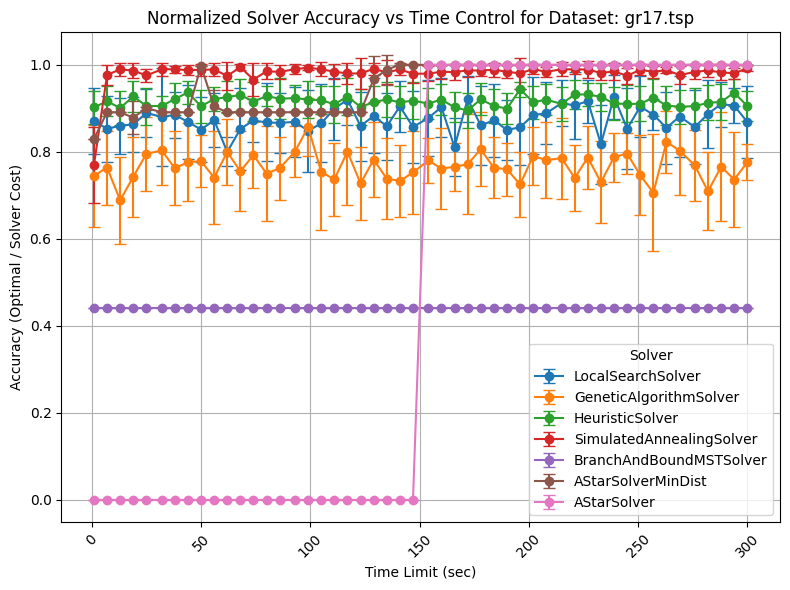
\includegraphics[width=0.7\linewidth]{figures/accuracy_line_gr17.tsp}
		\caption{}
		\label{fig:accuracylinegr17}
	\end{figure}
	\begin{figure}[H]
		\centering
		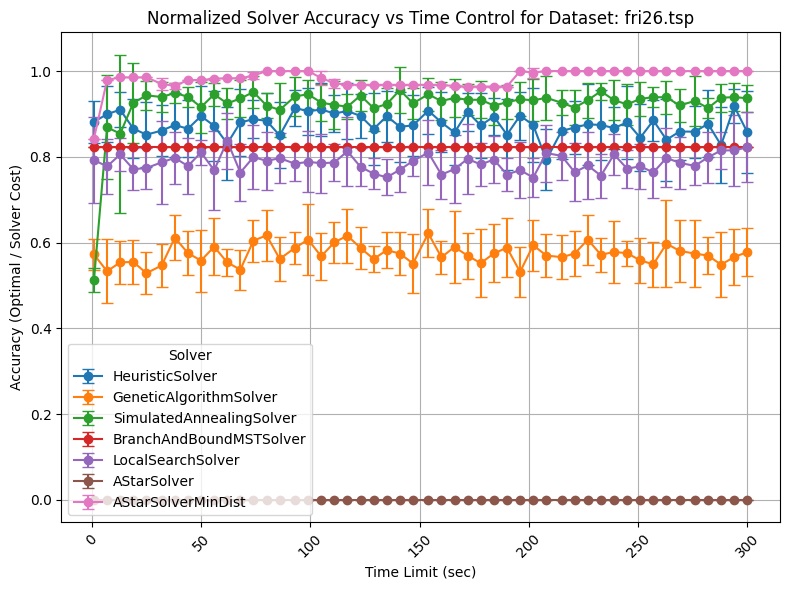
\includegraphics[width=0.7\linewidth]{figures/accuracy_line_fri26.tsp}
		\caption{}
		\label{fig:accuracylinefri26}
	\end{figure}
	\begin{figure}[H]
		\centering
		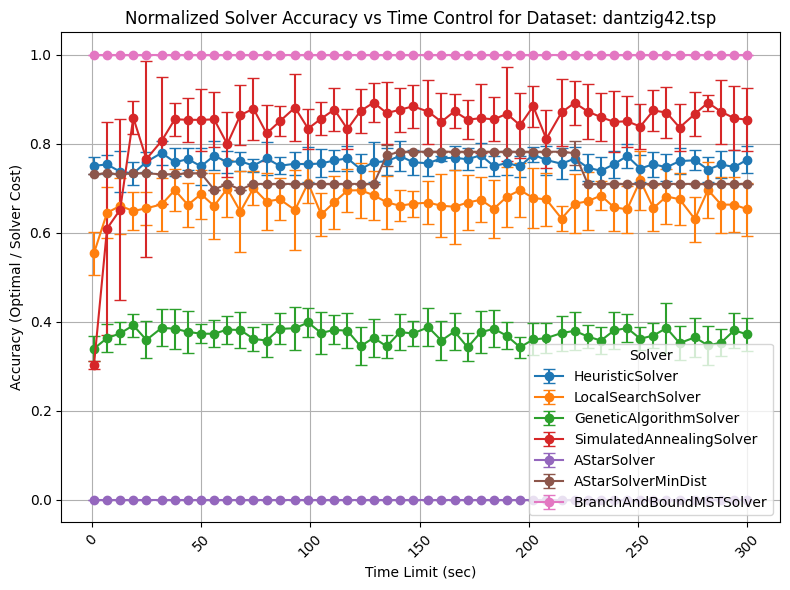
\includegraphics[width=0.7\linewidth]{figures/accuracy_line_dantzig42.tsp}
		\caption{}
		\label{fig:accuracylinedantzig42}
	\end{figure}
	\begin{figure}[H]
		\centering
		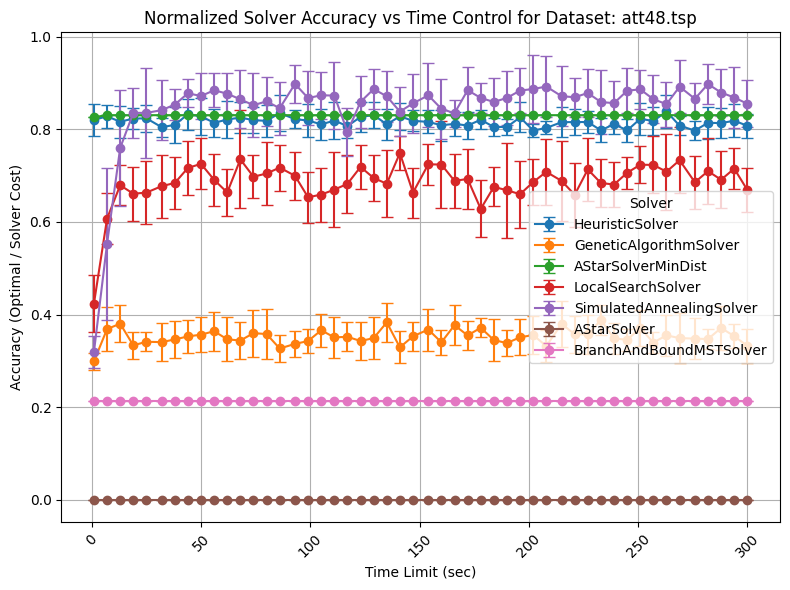
\includegraphics[width=0.7\linewidth]{figures/accuracy_line_att48.tsp}
		\caption{}
		\label{fig:accuracylineatt48}
	\end{figure}
	
	
	\begin{figure}[H]
		\centering
		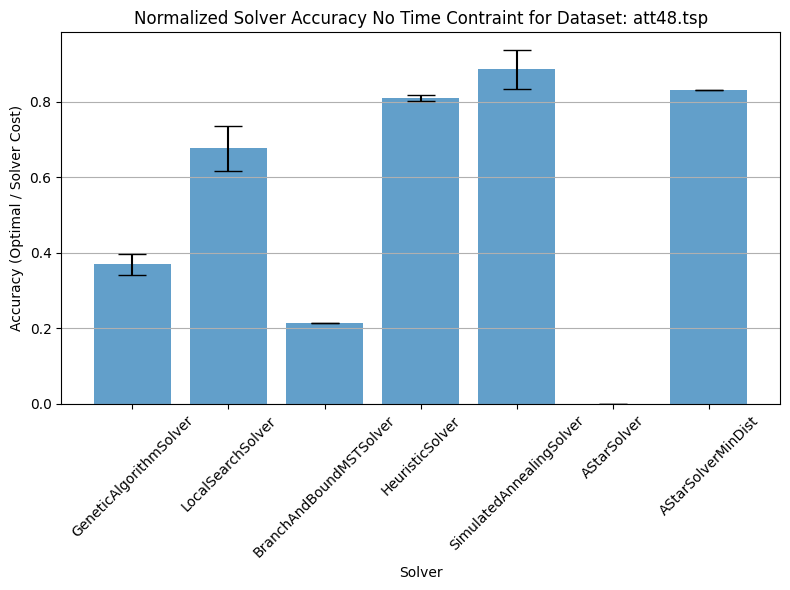
\includegraphics[width=0.7\linewidth]{figures/accuracy_bar_time0_att48.tsp}
		\caption{}
		\label{fig:accuracybartime0att48}
	\end{figure}
	\begin{figure}[H]
		\centering
		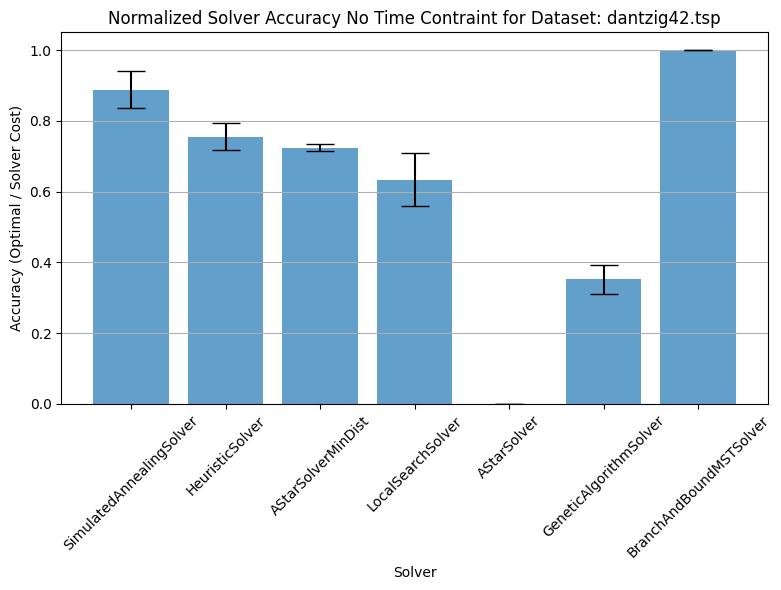
\includegraphics[width=0.7\linewidth]{figures/accuracy_bar_time0_dantzig42.tsp}
		\caption{}
		\label{fig:accuracybartime0dantzig42}
	\end{figure}
	\begin{figure}[H]
		\centering
		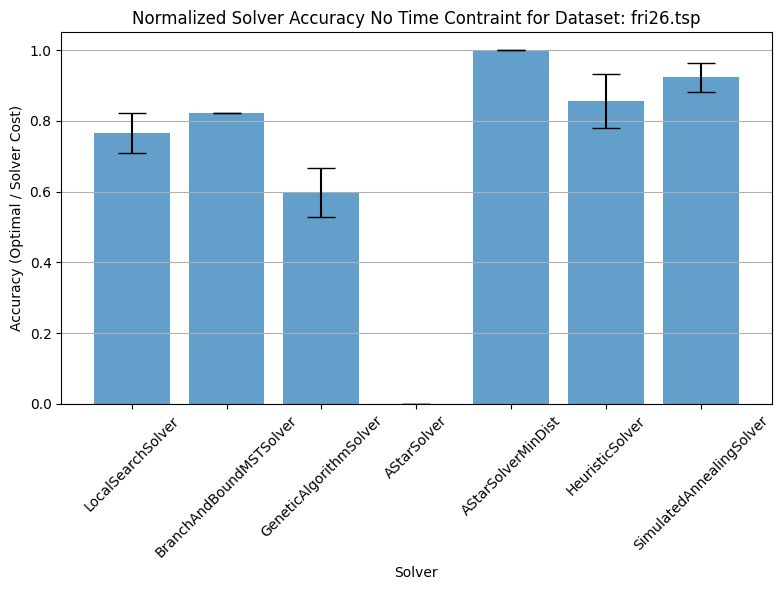
\includegraphics[width=0.7\linewidth]{figures/accuracy_bar_time0_fri26.tsp}
		\caption{}
		\label{fig:accuracybartime0fri26}
	\end{figure}
	\begin{figure}[H]
		\centering
		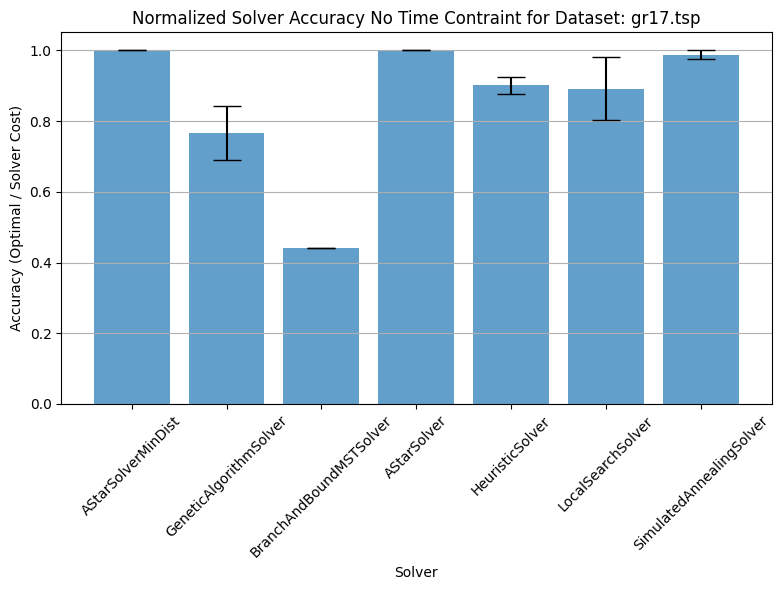
\includegraphics[width=0.7\linewidth]{figures/accuracy_bar_time0_gr17.tsp}
		\caption{}
		\label{fig:accuracybartime0gr17}
	\end{figure}
	\begin{figure}[H]
		\centering
		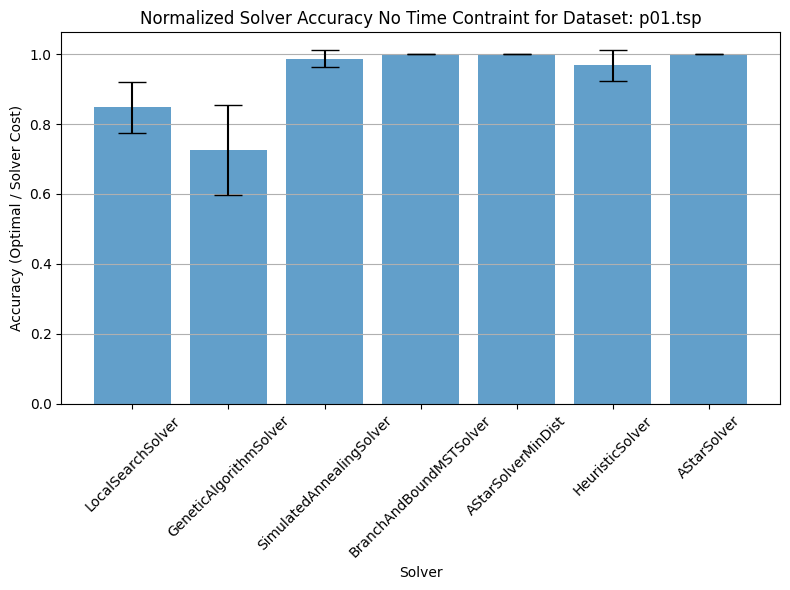
\includegraphics[width=0.7\linewidth]{figures/accuracy_bar_time0_p01.tsp}
		\caption{}
		\label{fig:accuracybartime0p01}
	\end{figure}
	
	
	\section{Discussion}
	The experimental findings reveal significant differences in algorithm performance and their sensitivity to additional computational time:
	
	\subsection{Heuristic-Based Methods}	
	\subsubsection{Simple Heuristic, Minimum Distance}
	The Minimum Distance heuristic provided solutions rapidly. However, due to its non-iterative nature, more runtime does not enhance the solution quality. Its performance remains static regardless of additional time beyond initial solution generation (which is effectively linear with number of cities). To make this a bit more Competitive, random starting locations were implemented. However, the earlier limitation still applies; upon completion of a solution, additional time does not improve solution quality.
	
	\subsubsection{Graph-Based A Star Search}
	A* produces optimal solutions given enough time, it is not inherently an anytime algorithm. Its solution quality does not improve incrementally; instead, the complete solution is only available once the entire search has been conducted. Under tight deadlines, A* fails to complete the full search, providing no valid solution. And this is readily apparent for larger datasets as observed, where there is simply not enough time to produce any path at all. Note, on the largest dataset, A* requires multiple days to produce a valid path on the experiment's hardware.
	
	\subsubsection{Graph-Based A Star Search with Minimum Distance Fallback}
	A* begins attempting to find a path; once the time limit is reached, the current best path is then completed using minimum distance search. Under tight deadlines, this method produces similar results to the simple minimum distance heuristic search. However, this method takes advantage A* when more generous time constraints are allowed, identifying a better initial path portion than the purely greedy approach.
	
	\subsubsection{Tree-Based Branch and Bound with MST} 
	The Branch and Bound approach appears to always deliver a final valid solution after exploring a minimal portion of the search space. With additional time, it does not provide improvements. Since the depth is reached even in tight timing constraints, this algorithm is effective at all timescales tested, and sometimes even optimal.
	
	\subsection{Local Search-Based Methods}
	\subsubsection{Standard Local Search}
	This method always returns a complete solution, and its quality improves incrementally with additional time as it continues to explore the solution space. However, it tends quickly converge to a local minimum. This can be seen in the standard deviation in the plots. A notable benefit of using the standard implementation is no hyper parameter configuration to achieve the observed results. 
	
	\subsubsection{Genetic Algorithm} 
	The GA continuously maintains a population of valid solutions. Given more time, it evolves better candidates through successive generations, offering clear incremental improvements. Its anytime nature makes it well-suited for scenarios with varying time constraints. However, it is highly dependent on the hyper parameters. Requiring tuning if used in a production setting.
	
	\subsubsection{Simulated Annealing} 
	Starting from a complete solution, SA improves iteratively as the cooling schedule allows exploration of different regions in the solution space. With additional time, the likelihood of escaping local minima increases, enhancing solution quality. Note this method is also dependent on hyper parameters, but is fairly robust over longer and longer time controls.
	
	\subsection{Overall Observations}
	The experiments confirm that anytime algorithms—those that always return a valid solution and gradually improve it (e.g., Local Search, Genetic Algorithm, and Simulated Annealing)—are more robust under deadline constraints. In contrast, algorithms like A* and Branch and Bound require complete execution to yield their optimal solutions and are less effective when limited by time.
	
	\subsection{Related work}
	Other authors demonstrate improvements applied to local search style algorithms, targeting better selection strategies \cite{8367362}\cite{6492788}. This work focuses primarily on deadline impact to accuracy for a range of algorithms. In addition we propose an enhancement to a traditionally inapplicable algorithm for TSP due to exponential growth of the problem space.
	
	\section{Conclusions and Future Work}
	This survey examined several approaches to the TSP under deadline constraints, focusing on how solution quality is affected by available computation time. Key conclusions include:
	\begin{itemize}[noitemsep]
		\item \textbf{Anytime vs. Complete Search Algorithms:} Anytime algorithms, which continuously refine a complete solution, are advantageous under longer time constraints. In contrast, methods that require a complete node-by-node construction (like A* and Branch and Bound) may fail to produce useful solutions if interrupted.
		\item \textbf {Enhanced Complete Search Algorithms:} Conversion of a complete search algorithm to meet time constraints allows normally failing algorithms to produce valid solutions with improved performance. A* with minimum search heuristic fallback demonstrates this clearly.
		\item \textbf{Incremental Improvement:} For algorithms such as Genetic Algorithms and Simulated Annealing, additional computational time typically results in better solutions as the search space is explored more thoroughly. This improvement is gradual and observable over multiple iterations. There's a timescale where these methods generally perform better, and before this timescale, heuristics dominate.
		\item \textbf{Scalability Issues:} As problem size increases, even anytime algorithms face challenges in finding near-optimal solutions quickly, highlighting the need for efficient parallelization and hybrid strategies.
	\end{itemize}
	
	Future work could explore hybrid approaches that combine the rapid initial solution of heuristics with the refinement capabilities of local search methods. Alternatively, augmenting existing greedy approaches to improve given additional time would be a good area of research. (This is in effect what most local search algorithms are doing.) Additionally, adaptive strategies that dynamically allocate computational resources based on the current solution quality may further enhance performance under varying deadline constraints.
	
	\section{Appendix}
	Complete source code to reproduce these results are available online at\\
	 \texttt{https://github.com/allesrebel/cs271-project}\cite{allesrebel_cs271project}.
	
	% Auto generates References Section
	\bibliographystyle{ieeetr}
	\bibliography{references.bib}
	
\end{document}
